\documentclass[preprint,12pt,number]{elsarticle}

\usepackage[T1]{fontenc}
\usepackage[utf8]{inputenc}
\usepackage[a4paper,top=2.4cm,bottom=2.4cm,left=2.4cm,right=2.4cm]{geometry}
\usepackage{amsmath,amssymb}
\usepackage{booktabs}
\usepackage{graphicx}
\usepackage{float}
\renewcommand{\topfraction}{0.9}
\renewcommand{\bottomfraction}{0.7}
\renewcommand{\textfraction}{0.1}
\renewcommand{\floatpagefraction}{0.75}
\setcounter{topnumber}{3}
\setcounter{totalnumber}{4}
\usepackage{url}
\usepackage[hidelinks]{hyperref}
\usepackage{orcidlink} 
\journal{SoftwareX}

\begin{document}

\begin{frontmatter}

\title{\texttt{LQL-Equiv-Web}: a Browser-Based Implementation of Linear-Quadratic-Linear Dose Equivalence for Radiotherapy}

\author[label1]{Cyril Voyant\corref{cor1}\orcidlink{0000-0003-0242-7377}}
\ead{cyril.voyant@minesparis.psl.eu}
\author[label2]{Daniel Julian}
\ead{Julian@ccgm.fr}

\affiliation[label1]{organization={Mines Paris, PSL University},
            addressline={Centre for observation, impacts, energy (O.I.E.)},
            city={Sophia-Antipolis},
            postcode={06904},
            state={Antibes},
            country={France}}
\cortext[cor1]{Corresponding author}
\affiliation[label2]{organization={Centre de Canc\'erologie du Grand Montpellier},
            addressline={Radiotherapy Unit},
            city={Montpellier},
            postcode={34000},
            state={H\'erault},
            country={France}}

\begin{abstract}
Dose equivalence calculations decide how radiotherapy schedules are compared, compensated after an interruption, and summed in reirradiation. They are also applied inconsistently: across identical clinical cases, inter-practitioner agreement reaches only 25.8\,\% and nearly half of surveyed centres report no
usable tool. \texttt{LQL-Equiv} computes biologically effective dose, equivalent dose in a reference fractionation, normal-tissue complication probability, tumour control probability and radiation-induced cancer risk under the linear-quadratic-linear model, with corrections for incomplete inter-fraction repair, accelerated proliferation and treatment protraction, over any number of successive courses separated by gaps. Version~3.0 is a dependency-free Python library and a browser application that runs entirely on the user's machine through \texttt{WebAssembly}: no installation, no licence fee, and no computation on a server. It was regression-tested case by case against the 2014 \texttt{MATLAB} reference implementation over 4438 treatment schedules, agreeing on 69\,125 of 69\,131 compared values, its solver was checked against the original exhaustive search over 10\,554 searches, and its equations are pinned independently of both by closed-form tests. The complication and control probabilities are point estimates on a single equivalent dose and have not been validated against clinical outcome. It is intended for research and education and is not a medical device.
\end{abstract}

\begin{keyword}
Radiotherapy \sep Biologically effective dose \sep Linear-quadratic-linear model \sep \texttt{NTCP} \sep \texttt{TCP}  
\end{keyword}

\end{frontmatter}

%% ---------------------------------------------------------------------------
\section*{Code metadata}

\begin{table}[h!]
\centering
\small
\begin{tabular}{@{}lp{4.6cm}p{7.0cm}@{}}
\toprule
\textbf{Nr} & \textbf{Code metadata description} & \textbf{Metadata} \\
\midrule
C1 & Current code version & v3.0.0, commit \texttt{dda60cb} \\
C2 & Permanent link to code/repository & \url{https://github.com/cyrilvoyant/LQL-Equiv-web} \\
   & \quad archived release & \url{https://doi.org/10.5281/zenodo.21948623} \\
   & \quad running application & \url{https://cyrilvoyant.github.io/LQL-Equiv-web/} \\
C3 & Legal code license & MIT License \\
C4 & Code versioning system used & git \\
C5 & Software code languages, tools and services used & Python 3.10+, Streamlit, Altair, Pandas; stlite/Pyodide (WebAssembly);
     GitHub Actions; GitHub Pages \\
C6 & Compilation requirements, operating environments and dependencies & Any modern web browser for the hosted application. As a library:
     Python $\geq$ 3.10, standard library only. Linux, macOS, Windows \\
C7 & Link to developer documentation/manual & \url{https://github.com/cyrilvoyant/LQL-Equiv-web/blob/main/README.md} \\
C8 & Support email for questions & cyril.voyant@minesparis.psl.eu \\
\bottomrule
\end{tabular}
\caption{Code Metadata.}
\label{tab:metadata}
\end{table}

%% ---------------------------------------------------------------------------
\section{Motivation and Significance}
Radiotherapy schedules that differ in fraction size, fraction number or overall time cannot be compared by adding up physical dose: 20~$\times$~3\,Gy and
30~$\times$~2\,Gy are both 60\,Gy and are not the same treatment. The comparison is made through the biologically effective dose and the equivalent dose in a
reference fractionation, usually 2\,Gy per fraction (\texttt{EQD2}) \cite{fowler1989,fowler2010,jones2001,bentzen2012,voyant2017}. These quantities govern three decisions taken in every department: how to compensate an unscheduled interruption \cite{rcr2019,jones2020,oshea2022}, whether a hypofractionated schedule is acceptable, and how to accumulate dose in reirradiation \cite{appelt2026,hardcastle2024}. The calculation is not applied consistently. In a structured workshop where radiation oncologists, medical physicists and technologists applied the same models to the same standardized cases, mean inter-practitioner agreement reached 25.8\,\% (Jaccard index), falling to 10\,\% for head-and-neck cases; proposed dose-per-fraction adjustments for identical situations ranged from 1.8 to 2.5\,Gy, and nearly half of the surveyed centres reported that they could not compute biologically equivalent schedules with the tools available to them \cite{voyant2026standard,voyant2025}. Multi-centre studies of reirradiation reach the same conclusion from a different direction: intercentre variation in radiobiological dose scaling introduces clinically relevant differences in cumulative dose \cite{wahlstedt2026,hardcastle2024,stroom2025}. 

Part of that dispersion is not disagreement about radiobiology but about vocabulary. Identical parameters yield substantially different reported \texttt{EQD2}
values depending on whether proliferation is applied to the evaluated schedule only or symmetrically to the evaluated and the reference schedule. Three modelling elements are needed and are routinely omitted. First, the linear-quadratic model is widely held to overestimate cell kill at the fraction sizes used in stereotactic treatments, although the evidence is tissue- and endpoint-dependent and the point is not settled \cite{astrahan2008,guckenberger2013,brown2014}; the linear-quadratic-linear (\texttt{LQL}) form of \texttt{Astrahan} replaces the quadratic term by a straight line above a transition dose. Second, overall treatment time matters: accelerated proliferation after a kick-off time consumes dose every day, so an interruption is not neutral \cite{withers1988,dale1989,dale2024}. Third, two fractions a day require the incomplete repair correction \cite{thames1985}. A tool that omits any of the three cannot answer the questions above under these model assumptions; a deliberately simpler model can of course answer a narrower question. 

Software implementing these models exists \cite{jaikuna2017,tzikas2024,singh2018,yusoff2016,calvo2026}, and was published in 2014 \cite{voyant2014,lqlequiv2014soft}. That release was a \texttt{MATLAB GUIDE} application distributed as a Windows executable requiring the \texttt{MATLAB Component Runtime}. The barrier was practical rather than scientific: a several hundred megabyte runtime, a single operating system, an interface in French, and 3567 lines of source in which the entire calculation sat inside one callback. It could not be inspected, cited by version, or run by a colleague in a browser during a meeting. \texttt{LQL-Equiv}~3.0 removes that barrier without discarding the validated model. It is a reimplementation of the same calculation as a dependency-free Python library and a browser application, validated case by case against the original, with the provenance of every radiobiological parameter recorded.

\section{Software Description}
The package follows a \texttt{src} layout and separates three concerns. The core, \texttt{src/lqlequiv/}, contains the model (\texttt{model.py}), the calendar conversion (\texttt{schedule.py}) and the radiobiological library (\texttt{tissues.py}, backed by \texttt{data/tissues.json}); it depends only on the \texttt{Python} standard library, which keeps it auditable and makes it light enough to ship to a browser. 

\subsection{Architecture}
The interface, \texttt{app/streamlit\_app.py}, is a \texttt{Streamlit} application. The delivery layer, \texttt{tools/build\_stlite.py}, embeds the sources into a single \texttt{HTML} page of about 112\,kB, which loads a version-pinned \texttt{stlite} \cite{stlite} that in turn runs \texttt{Streamlit} on \texttt{Pyodide} \cite{pyodide}; the page carries the model but not the runtime. \texttt{GitHub} Actions rebuilds and publishes that page on every push; the whole cycle takes about 25\,s. The consequence is architectural rather than cosmetic (Fig.~\ref{fig:interface}). No computation happens on a server: each visitor browser downloads static files and executes the model locally. The precise claim, since it matters when a physicist types a real patient schedule, is this: the page embeds the model source itself, fetches the version-pinned \texttt{stlite} and \texttt{Pyodide} runtime from a public content delivery network on first load, carries no analytics and submits no form. 
    \begin{figure}
    \centering
    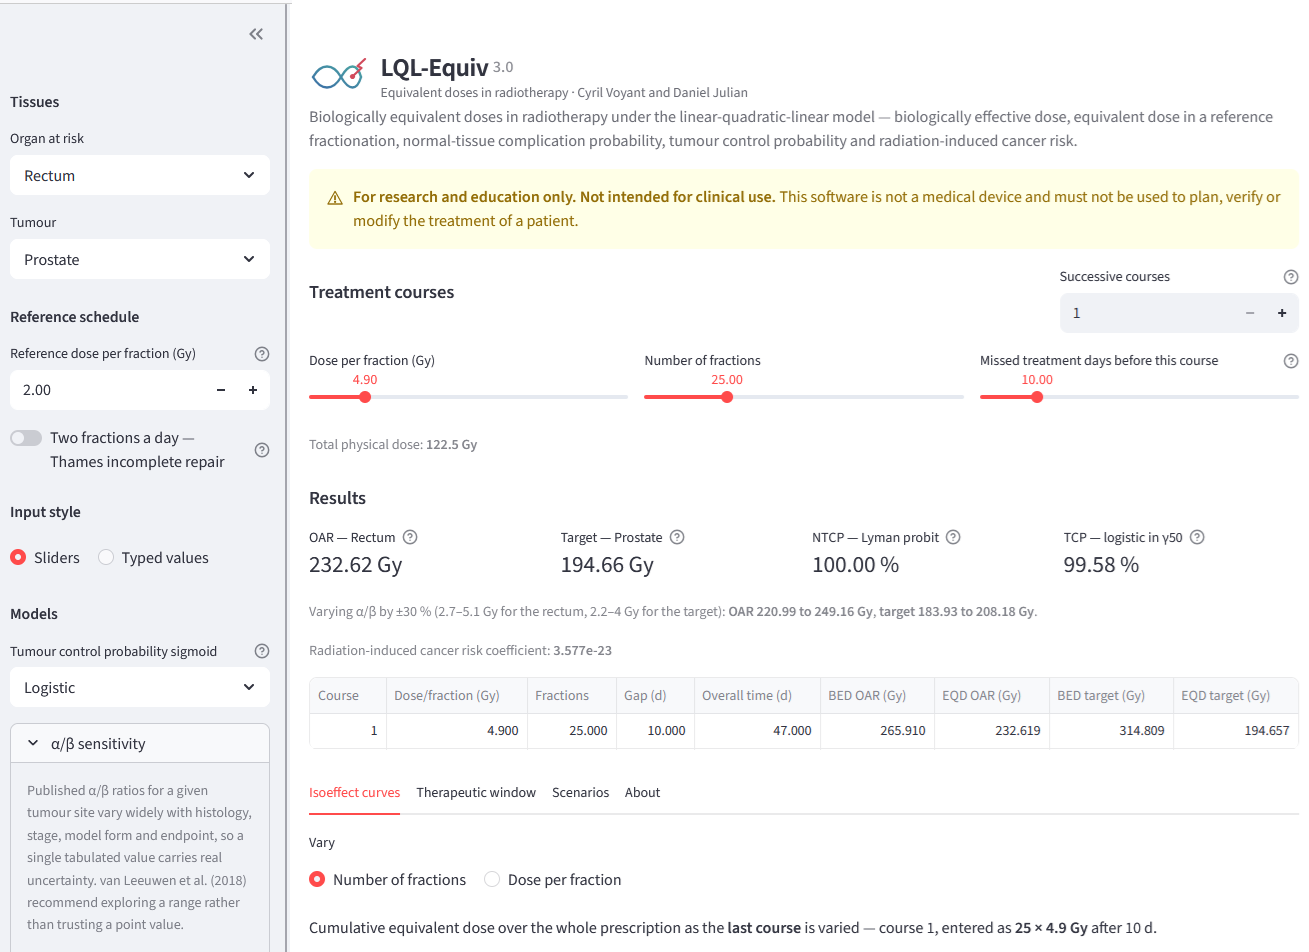
\includegraphics[width=\textwidth]{figures/fig4_interface.png}
    \caption{The application running in a browser, with nothing installed. Left, the tissue library and the choice of sigmoid; centre, the courses and the resulting equivalent doses, complication and control probabilities, with the $\alpha/\beta$ interval reported beneath them.}
    \label{fig:interface}
    \end{figure}

\subsection{Formulation} \label{sec:formulation}
A course delivers $n$ fractions of dose $d$ (Gy) and spans an overall time $T$ (days).

\subsubsection{Notation}
Each tissue carries seven parameters (listed in Table~\ref{tab:notation}) and the dose lost per day to proliferation is estimated by
    \begin{equation}
    D_\mathrm{prol} \;=\; \frac{\ln 2}{\alpha\,T_p} \qquad (\mathrm{Gy\,d^{-1}}).
    \label{eq:dprol}
    \end{equation}
    
    \begin{table}
    \centering
    \small
    \begin{tabular}{@{}llll@{}}
    \toprule
    Symbol & Meaning & Unit & Model \\
    \midrule
    $\alpha/\beta$ & sensitivity ratio & Gy & linear-quadratic \\
    $\alpha$ & linear coefficient & Gy$^{-1}$ & linear-quadratic \\
    $d_t = 2\,\alpha/\beta$ & transition dose, above which the response is linear & Gy & \texttt{LQL} \\
    $\gamma/\alpha$ & slope of the linear tail & --- & \texttt{LQL} \\
    $T_{1/2}$ & repair half-time & h & incomplete repair \\
    $T_k$ & kick-off time of accelerated proliferation & d & proliferation \\
    $T_p$ & effective doubling time & d & proliferation \\
    \bottomrule
    \end{tabular}
    \caption{Tissue parameters.}
    \label{tab:notation}
    \end{table}

\subsubsection{Two Fractions a Day}
For $m$ fractions a day separated by $\Delta t$, the incomplete-repair correction of Thames \cite{thames1985} applies:
    \begin{equation}
    H_m \;=\; \frac{2\varphi}{m}\,\frac{1}{1-\varphi} \left[\,m - \frac{1-\varphi^{m}}{1-\varphi}\right], \qquad \varphi = \exp\!\left(-\frac{\ln 2\,\Delta t}{T_{1/2}}\right).
    \label{eq:hm}
    \end{equation}
At most two fractions a day are allowed, six hours apart. For $m = 2$ the bracket becomes $1-\varphi$, so \eqref{eq:hm} reduces to
    \begin{equation}
    H_2 \;=\; \varphi \;=\; 2^{-\Delta t / T_{1/2}}, \qquad \Delta t = 6\,\mathrm{h},
    \label{eq:h2}
    \end{equation}
and $H_1 = 0$ for one fraction a day. The correction is defined on the quadratic branch only, so it is dropped above the transition dose. A twice-daily course is therefore admissible only when $d$ lies below the transition doses of both selected tissues, and the software refuses the combination otherwise rather than returning a value with the repair term silently missing. Note that $m$ counts fractions per day here; it is not the Lyman parameter of Eq.~\eqref{eq:ntcp}. In Eqs.~\eqref{eq:dprol} and \eqref{eq:hm} the rounded constant $0.693$ is used, as in the 2014 release, rather than $\ln 2$.

\subsubsection{Biologically Effective Dose}
The response is linear-quadratic below the transition dose and linear above it. Proliferation is subtracted once the overall time passes $T_k$:
    \begin{equation}
    \texttt{BED}(d,n,T) =
    \begin{cases}
    \; n\,d\left[1 + \dfrac{(1+H_m)\,d}{\alpha/\beta}\right] - D_\texttt{prol}\,(T-T_k)_{+}, & d < d_t,\\[2.2ex]
    \; n\left[d_t\left(1 + \dfrac{d_t}{\alpha/\beta}\right)  + \dfrac{\gamma}{\alpha}\,(d-d_t)\right] - D_\texttt{prol}\,(T-T_k)_{+}, & d \geq d_t,
    \end{cases}
    \label{eq:bed}
    \end{equation}
with $(x)_{+} = \max(x,0)$. The two branches are tied together. Below $d_t$ the slope in $d$ is $1 + 2d/(\alpha/\beta)$. Requiring the linear tail to join it smoothly therefore fixes
    \begin{equation}
    \frac{\gamma}{\alpha} \;=\; 1 + \frac{2\,d_t}{\alpha/\beta} \qquad \text{when } d_t = 2\,\alpha/\beta .
    \label{eq:continuity}
    \end{equation}
The value given by Eq.~\eqref{eq:continuity} is therefore not a free parameter: always equal to $5$, it follows from the choice $d_t = 2\,\alpha/\beta$, which is the convention of the 2014 library \cite{voyant2014}. Astrahan treats $d_t$ as fitted to the tissue \cite{astrahan2008}. The two tissues do not share one proliferation model, and the difference is deliberate. For the target volume, nothing is lost before $T_k$ \cite{dale1989,withers1988}. For the organ at risk, a recovered dose accrues from the first day and $T_k$ is not read at all \cite{vandyk1989}.

\subsubsection{Equivalent Dose}
Let $d_r$ be the reference dose per fraction, usually 2\,Gy. The equivalent dose is the dose of a reference schedule carrying the same biologically effective dose. The fraction count $n_r$ solves
    \begin{equation}
    \;\texttt{BED}\big(d_r,\,n_r,\,T(n_r)\big) \;=\; \texttt{BED}\big(d,\,n,\,T(n)\big)\;
    \label{eq:core}
    \end{equation}
and the answer is read off as
    \begin{equation}
    \texttt{EQD}_{d_r} \;=\; n_r\,d_r .
    \label{eq:eqd}
    \end{equation}
Two points about Eq. \eqref{eq:core} account for most of the disagreement between implementations. First, the reference schedule on the left carries its own overall time, and therefore its own proliferation loss. A definition that corrects only the right-hand side answers a different question and returns a different number. Second, nothing is added after \eqref{eq:eqd}. In the special (and usual) case with $d_r=2$ Gy \texttt{EQD} is noted \texttt{EQD2} and is computed via $2n_r$.

\subsubsection{Treatment calendar}
Overall time is not the fraction count. Treatment runs five days a week, and $m$ fractions a day occupy $\lceil n/m \rceil$ sessions. Sessions accumulate across courses, and $s$ sessions span
    \begin{equation}
    \Theta(s) \;=\;
    \begin{cases}
    s, & s < 6,\\[0.8ex]
    s + 2\left(\left\lfloor \dfrac{s-6}{5} \right\rfloor + 1\right), & s \geq 6,
    \end{cases}
    \qquad
    s_j \;=\; \sum_{i \leq j}\left(\left\lceil \frac{n_i}{m} \right\rceil + g_i\right),
    \label{eq:time}
    \end{equation}
calendar days, weekends included, where $g_i$ is the number of sessions missed before course $i$. A course occupies the increment $\Theta(s_j) - \Theta(s_{j-1})$. Ten fractions given twice a day occupy five sessions and therefore span $\Theta(5) = 5$ days, against $\Theta(10) = 12$ days once a day. Because gaps are counted in missed sessions, the weekends inside an interruption are supplied by $\Theta$ itself. Public holidays and a course starting mid-week are not modelled. Proliferation is charged per elapsed day, and cells do not rest at the weekend, so Eq. \eqref{eq:time} enters both sides of Eq.\eqref{eq:core}. This makes the equality a step function in $n_r$, with no closed form over the whole range. It has one on each interval between two weekends, where $\Theta(s) = s + \text{constant}$ and the loss is linear in $n_r$; every interval is solved and the best root kept. Where a target falls inside one of the two-day jumps, two fraction counts satisfy it exactly and the shorter is reported, so that the equivalent dose stays a function of its input.

\subsubsection{Successive Courses}
The reference schedule is not restarted at each course. Writing $\tau_j$ for the reference time already spent before course $j$, with $\tau_1 = 0$, the software solves
    \begin{equation}
    \texttt{BED}\big(d_r,\,n_{r,j};\,\tau_j,\,\tau_j + \Theta(n_{r,j})\big) \;=\; \texttt{BED}\big(d_j,\,n_j;\,\Theta(s_{j-1}),\,\Theta(s_j)\big), \qquad \tau_{j+1} = \tau_j + \Theta(n_{r,j}),
    \label{eq:multi}
    \end{equation}
so that each course is matched against the segment of one continuous reference schedule that follows the segments already spent. Proliferation is then subtracted once over the total elapsed time, and the equivalent doses add, $\texttt{EQD} = \sum_j n_{r,j}\,d_r$. Additivity holds because the losses telescope across consecutive segments.

\subsubsection{Complication and Control Probabilities}
Both follow from the cumulative equivalent dose. The complication probability uses the \texttt{Lyman} probit \cite{lyman1985}, with $D_{50}$ the dose giving a 50\,\% complication rate and $m$ a dimensionless dispersion parameter, inversely related to the steepness of the response:
    \begin{equation}
    \texttt{NTCP} = \frac{1}{2}\left[1 + \operatorname{erf} \left(\frac{u}{\sqrt{2}}\right)\right], \qquad u = \frac{\texttt{EQD} - D_{50}}{m\,D_{50}} .
    \label{eq:ntcp}
    \end{equation}
The control probability uses a logistic sigmoid through $\texttt{TCD}_{50}$, the dose controlling half of tumors, with normalized slope $\gamma_{50}$:
    \begin{equation}
    \texttt{TCP} = \left[1 + \left(\frac{\texttt{TCD}_{50}}{\texttt{EQD}}\right)^{4\gamma_{50}} \right]^{-1}.
    \label{eq:tcp}
    \end{equation}
A Poisson form, $\texttt{TCP} = 2^{-\exp[e\,\gamma_{50}(1 - \texttt{EQD}/\texttt{TCD}_{50})]}$, is also offered; it shares the same two parameters and differs in the tails. The choice is reported with the value. The radiation induced cancer risk follows a linear-exponential form, with $P$ and $\alpha_2$ in Gy$^{-1}$:
    \begin{equation}
    K = P\,\texttt{EQD}\,e^{-\alpha_2 \texttt{EQD}} ,
    \label{eq:risk}
    \end{equation}
$K$ being a dimensionless excess incidence on the scale of the fitted $P$, not an absolute lifetime risk.

\subsection{Functionalities}
For a chosen organ at risk, a chosen target volume and a sequence of successive courses each with its own fraction size, fraction number and preceding gap, the
software computes: 
    \begin{itemize}
      \item the biologically effective dose, linear-quadratic below the transition dose $d_t = 2\,\alpha/\beta$ and linear above it \cite{astrahan2008};
      \item the loss to proliferation, accumulated across courses and gaps, under the two models the tissues take: switched on at the kick-off time $T_k$ for 
            the target \cite{dale1989,withers1988}, and accruing from the first day for the organ at risk \cite{vandyk1989};
      \item the incomplete-repair correction for two fractions a day, six hours apart \cite{thames1985};
      \item the equivalent dose in any reference fractionation, for the organ at risk and for the target;
      \item the normal-tissue complication probability, \texttt{Lyman probit} \cite{lyman1985,burman1991};
      \item the tumour control probability, logistic or Poisson sigmoid in $\gamma_{50}$;
      \item the radiation-induced cancer risk under a linear-exponential model.
    \end{itemize}
The shipped library holds 34 organs at risk and 20 target sites. Nineteen of the latter are transcribed from the 2014 release; the twentieth was added in 3.0, a
standard tumor with proliferation switched off, which isolates the effect of fractionation from the effect of overall time. The interface offers sliders or typed entry, an isoeffect sweep over fraction number or fraction size, a therapeutic window in both directions, scenario comparison with \texttt{CSV} and \texttt{JSON} export, and an $\alpha/\beta$ sensitivity band. That last feature follows the systematic review of published $\alpha/\beta$ values, which recommends exploring a range rather than trusting a point estimate \cite{vanleeuwen2018}.

\subsection{Historical Multicentre Evaluation}
The model was evaluated across centres when it was first published \cite{voyant2014}: eight clinical calculators in seven French radiotherapy centres converted the same standard schedules, and did not agree. Relative standard deviations reached 17.7\,\% for the spinal cord and 29.6\,\% for a prostate metastasis on a single 8\,Gy fraction, stayed above 5\,\% on conventional 10~$\times$~3\,Gy schedules, and most centres could not compute a schedule containing a gap at all; the 2014 outputs were also compared against TDF~Plan \cite{tdfplan} schedule by schedule. That comparison against external calculators was not repeated for version 3.0. The survey is twelve years old and its finding has not aged \cite{voyant2026standard,wahlstedt2026,hardcastle2024}, but it bears on the 2014 application and is context, not evidence for the present release. What follows verifies that version~3.0 computes what the evaluated implementation computed, which is a claim about fidelity, and then checks the equations against closed forms, which is a claim about correctness. Neither is a clinical validation.

\subsection{Numerical Verification of Version 3.0} \label{sec:verification}
Two questions are asked separately here, and confusing them is easy. The first is whether the calculation was transcribed correctly from \texttt{MATLAB} to \texttt{Python}. The second is whether the transcribed calculation is right. This section answers the first, by switching the time handling of Section~\ref{sec:release} back to its 2014 form so that only arithmetic differences remain. Everything the software returns uses the current form. The transcription is exact. Over the 11\,505 organ equivalent doses that the 2014 search resolved rather than truncating at its bound, every value agrees to the six digits \texttt{MATLAB} prints. On the target side, 11\,663 of 11\,667 agree, the remaining four differing by 0.02\,Gy where the exact root falls halfway between two grid points and the original answer turns on floating-point noise. Nothing in Section~\ref{sec:release} rests on this comparison; it establishes only that the port introduced no error of its own, which is the necessary first step before any change can be attributed to a change of model. The 2014 application still runs under \texttt{MATLAB R2025b} and can be driven without a display. \texttt{tools/matlab/sweep.m} opens the figure invisibly, sets the input fields, invokes the callbacks in the order the interface would, and reads the output fields back, over 4438 treatment schedules: every organ/target pair on a reference schedule, a wide fractionation grid from 1.2 to 20\,Gy per fraction and 1 to 100 fractions with gaps and two-fractions-a-day schedules, and 600 randomized multi-course plans. The captured outputs form \texttt{tests/data/golden.jsonl}, which the test-suite replays. \texttt{MATLAB} writes its interface fields with six significant digits, which sets the resolution at which the two implementations can be compared at all. At that resolution they agree on all but six values, belonging to two cases in which the exact root falls precisely halfway between two points of the original search grid, so that the 2014 answer is decided by floating-point noise at the fifteenth decimal. The consequence is a shift of one grid step in $n_r$, worth up to 0.04\,Gy on the equivalent dose, which is the largest deviation in Table~\ref{tab:validation}.
    \begin{table}
    \centering
    \small
    \begin{tabular}{@{}lr@{}}
    \toprule
    \textbf{Quantity} & \textbf{Value} \\
    \midrule
    Treatment schedules replayed              & 4438 \\
    Values compared, all outputs              & 69\,131 \\
    Agreeing at the reference's own precision & 69\,125 (99.991\,\%) \\
    Cases differing                           & 2 (0.05\,\%) \\[0.5ex]
    Paired equivalent doses                   & 34\,403 \\
    Bit-identical                             & 31\,657 (92.0\,\%) \\
    Differing by less than $10^{-10}$\,Gy     & 2294 (6.7\,\%), arithmetic rounding \\
    Differing by more                         & 452 (1.3\,\%), grid ties \\
    Median absolute difference                & 0\,Gy \\
    95th, 99th percentile                     & $7.1\times10^{-15}$, $2.0\times10^{-4}$\,Gy \\
    Largest single deviation                  & 0.04\,Gy \\
    Tolerance $\delta$, values clearing it    & 0.05\,Gy, 34\,403 of 34\,403 \\[0.5ex]
    Searches replayed against the full grid   & 10\,554 \\
    Disagreements with the exhaustive search  & 0 \\
    Closed-form tests, no reference in the loop & 16, of which 4 separate the two conventions \\
    Unit and non-regression tests             & 51 in total \\
    \bottomrule
    \end{tabular}
    \caption{The port, checked against the 2014 program. This table measures faithfulness of transcription, not what version 3.0 returns: the time handling of Section~\ref{sec:release} is switched off here, so that the only differences left are arithmetic. Table~\ref{tab:release-effect} gives what the software
    returns. Dataset: \texttt{tests/data/golden.jsonl}.}
    \label{tab:validation}
    \end{table}
Both implementations are deterministic, so there is no sampling process and no population to infer to. What is reported is the whole distribution of the absolute difference against a tolerance fixed in advance (Fig.~\ref{fig:agreement}, Table~\ref{tab:validation}). The tolerance is $\delta = 0.05$\,Gy, chosen because the smallest dose increment any of these decisions turns on is of the order of a tenth of a gray, and every one of the 34\,403 paired values clears it, the largest deviation being 0.04\,Gy. Both checks are reproducible by the reader without MATLAB: \texttt{pytest} runs the unit and non-regression suites against the shipped dataset, the full grid replay included.
    \begin{figure}
    \centering
    \includegraphics[width=\textwidth]{figures/fig1_agreement.pdf}
    \caption{Agreement between version 3.0 and the 2014 reference implementation over 4438 treatment schedules ($n = 34\,403$ paired equivalent doses). (a)~Distribution of the absolute difference, zero excluded, on logarithmic axes; it splits into arithmetic rounding near the double-precision epsilon and 452
    grid ties four orders of magnitude above it. (b)~The same values read cumulatively: 92.0\,\% are bit-identical and all 34\,403 fall below the
    tolerance $\delta = 0.05$\,Gy. No inferential statistic is computed, both implementations being deterministic.}
    \label{fig:agreement}
    \end{figure}
A second check does not depend on the \texttt{MATLAB} outputs. The original locates the equivalent fraction count by evaluating an objective at 20\,001 grid points and taking the minimum; version 3.0 solves the objective in closed form and scores only the grid points around each root. That shortcut is legitimate only if it lands on the same point every time, which is not obvious because proliferation switching on at $T_k$ makes the tumor objective piecewise linear, so it can
approach the target twice and its best grid point can lie next to the kink rather than next to a root.

\subsection{What Changed Between 2014 and 2026} \label{sec:release}
Software improves between releases, and the changes should be traced rather than assumed. Table~\ref{tab:release} lists them. Four are software; one changes a number.
    \begin{table}
    \centering
    \small
    \begin{tabular}{@{}lp{5.2cm}p{5.2cm}@{}}
    \toprule
     & \textbf{2014} & \textbf{2026, version 3.0} \\
    \midrule
    Delivery & Windows executable, MATLAB runtime & browser page, or Python library \\
    Source & one callback, 3567 lines & \texttt{src} layout, standard library only \\
    Search & 20\,001 grid points, stops at 100 fractions & closed form, no upper bound \\
    Interface & French, fixed fields & English, sliders or typed entry, export \\
    Control probability & parameters loaded, never used & computed and reported \\[0.8ex]
    \textbf{Overall time} & \textbf{partly counted} & \textbf{counted in full} \\
    \bottomrule
    \end{tabular}
    \caption{Changes between the two releases.}
    \label{tab:release}
    \end{table}
The last row is the one that moves results. The 2014 code handled overall time in two steps. It first solved \eqref{eq:core} with time charged at a flat rate of $7/5$ days per fraction. It then subtracted a further $(T - T_r)\,D_\mathrm{prol}$ from the answer, using the calendar of \eqref{eq:time} this time. The elapsed time is therefore charged twice, once inside the equality and once after it. Version 3.0 charges it once, on the calendar of \eqref{eq:time} throughout, and reports $n_r d_r$ as \eqref{eq:eqd} states. Weekends are included, since cells proliferate on Saturdays. Handling overall time is not obvious, in 2014 software its effect was to report more dose to an organ than the schedule carries, which made it the more conservative of the two. How much this matters depends on one parameter, $D_\texttt{prol}$, and Table~\ref{tab:release-effect} makes that visible by including a tissue for which it is zero. The spinal cord carries no recovered dose, so the time term is identically zero and the two versions cannot differ. They do not, at any fraction size. Everything seen on the other three is the time term and nothing else, and it scales with $D_\texttt{prol}$: the lung, at 0.54\,Gy per day, moves about twice as far as the rectum at 0.30.
    \begin{table}
    \centering
    \small
    \begin{tabular}{@{}lrrrrrrrr@{}}
    \toprule
     & \multicolumn{2}{c}{Spinal cord} & \multicolumn{2}{c}{Rectum}
     & \multicolumn{2}{c}{Heart} & \multicolumn{2}{c}{Lung} \\
    $D_\mathrm{prol}$ (Gy\,d$^{-1}$) & \multicolumn{2}{c}{0.00}
     & \multicolumn{2}{c}{0.30} & \multicolumn{2}{c}{0.30}
     & \multicolumn{2}{c}{0.54} \\
    \cmidrule(lr){2-3}\cmidrule(lr){4-5}\cmidrule(lr){6-7}\cmidrule(lr){8-9}
    Dose per fraction & 2014 & 2026 & 2014 & 2026 & 2014 & 2026 & 2014 & 2026 \\
    \midrule
    1.8\,Gy  & $0.0$ & $0.0$ & $-6.1$ & $-2.4$ & $-5.9$ & $-1.9$ & $-12.0$ & $-4.4$ \\
    2.0\,Gy  & $0.0$ & $0.0$ & $0.0$ & $0.0$ & $0.0$ & $0.0$ & $0.0$ & $0.0$ \\
    3.0\,Gy  & $0.0$ & $0.0$ & $+17.9$ & $+7.2$ & $+16.5$ & $+5.5$ & $+34.7$ & $+13.1$ \\
    6.0\,Gy  & $0.0$ & $0.0$ & $+32.8$ & $+13.2$ & $+28.8$ & $+9.6$ & $+64.9$ & $+24.8$ \\
    12.0\,Gy & $0.0$ & $0.0$ & $+37.8$ & $+15.1$ & $+32.8$ & $+11.0$ & $+74.2$ & $+28.0$ \\
    \bottomrule
    \end{tabular}
    \caption{What overall time adds to the organ equivalent dose, as a percentage of the same calculation with the recovered dose set to zero. Total physical dose is
    60\,Gy in every entry.}
    \label{tab:release-effect}
    \end{table}
Three readings follow. The effect is nil at the reference fraction size, where the two schedules span the same time. It grows with the departure from it, reaching $+38$\,\% for the rectum and $+74$\,\% for the lung under the 2014 treatment against $+15$\,\% and $+28$\,\% now. And it changes sign below 2\,Gy per fraction, where a protracted schedule loses dose rather than gaining it; there too the 2014 treatment overshot. Four smaller defects of the 2014 release were also fixed. Equivalent doses past 100 reference fractions were reported at the search bound and stopped responding to added dose. Nine parameters were displayed differently from those used in the computation, across seven tissues. The weekend calendar contradicted itself past 86 fractions. Complication probability was reported as 100\,\% for the five tissues carrying no Lyman parameters, through a division by zero, and is now reported as unavailable.
    \begin{figure}
    \centering
    \includegraphics[width=\textwidth]{figures/fig5_difference2014.pdf}
    \caption{The time term, charged once and twice. 60\,Gy physical in every schedule.}
    \label{fig:difference2014}
    \end{figure}
The 2014 behavior remains reachable in the library, so that a result published before 2026 can be recomputed. Section~S1 of the supplementary material sets the two calculations side by side and gives the round-trip criterion that separates them.

\subsection{Clinical plausibility} None of the above says whether the model matches clinical experience, and no test here can. What can be asked is whether
schedules that randomized trials compared directly come out where the trials placed them. Against 78\,Gy in 39 fractions, the software puts the ultra-hypofractionated arm of \texttt{HYPO-RT-PC} at 77.94\,Gy \cite{widmark2019hypo}, and it orders the two hypofractionated arms of \texttt{CHHiP} as the trial did, the one that met non-inferiority above the one that did not \cite{dearnaley2016chhip}. It also disagrees: 60\,Gy in 20 fractions comes out 5.5\,Gy below the
conventional arm of \texttt{PROFIT}, which demonstrated non-inferiority without hormone therapy \cite{catton2017profit}. That gap closes under $\alpha/\beta = 1.5$\,Gy, near the pooled clinical estimate of 1.4\,Gy \cite{miralbell2012alphabeta}, which is the clearest evidence that the tabulated 3.1\,Gy is not universal. On the organ side the tabulated Lyman parameters fail outright: 50\,Gy in 25 fractions to the spinal cord returns a complication probability of 5.1\,\% where \texttt{QUANTEC} puts the risk near 0.2\,\% \cite{kirkpatrick2010quantec}, a discrepancy also reported clinically \cite{daly2012lkb}.  Supplementary Section~S2 reports the complete external coherence checks against \texttt{HYPO-RT-PC}, \texttt{CHHiP}, \texttt{PROFIT}, \texttt{QUANTEC}, \texttt{HyTEC}, and \texttt{PACE-B} \cite{sahgal2021hytec}.

\subsection{Limitations}\label{sec:limitations}
The software is a model comparison tool and not a treatment planning system: it knows nothing of dose distribution, volume effects or plan constraints, and
voxel-level accumulation \cite{singh2018,calvo2026} is outside its scope. Two consequences follow for the toxicity endpoints and should be stated plainly.
Equation~\eqref{eq:ntcp} is a point estimate on a single equivalent dose, whereas the Lyman formalism is defined on a dose-volume histogram through an equivalent uniform dose \cite{niemierko1997} and is established near 2\,Gy per fraction; away from that fraction size, and for a serial organ where the relevant quantity is a near-maximum rather than a mean, it should be read as indicative. Equation~\eqref{eq:tcp} uses $\gamma_{50}$ and $\texttt{TCD}_{50}$ values that the 2014 library carried but never used, so the tumor control probability is newly exposed and unlike the equivalent dose, has not itself been validated against clinical outcome. The radiobiological library is the one published in 2014; its \texttt{Lyman} parameters fall in the range of the \texttt{Emami/Burman} fits \cite{emami1991,burman1991}, which is their probable but unverified origin, and the provenance of every value is recorded in \texttt{docs/PARAMETERS.md}. Model parameters carry uncertainty larger than many of the differences the software can display, which is why the $\alpha/\beta$ band exists and why the therapeutic window declines to name a best schedule when the uncertainty bars overlap. It is intended for research and education and is not a medical device. Stated operationally rather than generically, its outputs must not be used to choose or modify a prescription, to compute the compensation for a real interruption, to sum dose in a reirradiation decision, to accept or reject a treatment plan, to support a consent discussion, or to predict complication or control probability for an individual patient. What it is for is comparing schedules under a stated model, seeing how far that comparison moves when the assumptions move, and teaching why.

\section{Worked cases} \label{sec:examples}
Three cases are given. Each answers a question a department asks. The library is called in a few lines:
    \begin{verbatim}
    from lqlequiv import Course, Prescription, compute, load_library

    lib = load_library()
    plan = Prescription(courses=(Course(2.0, 39),), reference_dose=2.0)
    res = compute(lib.organ("Rectum"), lib.tumour_site("Prostate"), plan)

    res.eqd_oar_total   # 78.00 Gy EQD2 to the rectum
    res.ntcp_percent    # complication probability, proctitis
    res.tcp_percent     # tumour control probability
    \end{verbatim}

\subsection{What an Interruption Costs}
A course of 25~$\times$~2\,Gy reaches 50.00\,Gy \texttt{EQD2} on the standard tumor. Ten missed sessions add fourteen calendar days through Eq. \eqref{eq:time} and bring it down to 37.48\,Gy. The interruption costs 12.5\,Gy, more than six 2\,Gy fractions. Against the non-proliferating reference tumor the same interruption costs nothing, which separates the time effect from the fractionation effect. This is the quantity that compensation guidance asks a department to estimate \cite{rcr2019,jones2020,dale2024}.

\subsection{How Much the Model form Matters}
A department fixes the effect on the target and asks what the change costs the organ. In Table~\ref{tab:fractionation} the target receives 78\,Gy \texttt{EQD2} in every row, so only the organ moves. Fraction counts are whole numbers, so every row is deliverable.
    \begin{table}
    \centering
    \small
    \begin{tabular}{@{}llrr@{}}
    \toprule
    Target assumption & Schedule & Organ \texttt{EQD2} & Against 78\,Gy \\
    \midrule
    \texttt{LQ}, $\alpha/\beta = 1.5$\,Gy  & 5 $\times$ 6.65\,Gy & 67.49 & $-10.51$ \\
    \texttt{LQL}, $\alpha/\beta = 1.5$\,Gy & 5 $\times$ 8.42\,Gy & 100.08 & $+22.08$ \\
    \texttt{LQL}, tabulated 3.1\,Gy        & 5 $\times$ 7.55\,Gy & 83.79 & $+5.79$ \\
    \bottomrule
    \end{tabular}
    \caption{Five-fraction prostate schedules, iso-effective on the target.}
    \label{tab:fractionation}
    \end{table}
The three rows disagree on the sign. With a low $\alpha/\beta$ the transition dose falls to 3\,Gy, beneath every fraction size at issue, so the linear tail removes the target's advantage before it can be spent. The choice between \texttt{LQ} and \texttt{LQL} is therefore the largest single term in the answer, which is the reason a calculator must name the form it used.

This is a statement about three models, not about patients. The trial evidence decides the clinical question, and it is not in dispute: \texttt{HYPO-RT-PC} found non-inferior failure-free survival for 42.7\,Gy in 7 fractions \cite{widmark2019hypo}, and PACE-B found non-inferior control for 36.25\,Gy in 5, with more grade~2 or worse genitourinary toxicity at five years \cite{vanas2024paceb}. The complication percentages here come from a point dose with no volume information and must not be compared with measured toxicity.
    \begin{figure}
    \centering
    \includegraphics[width=\textwidth]{figures/fig2_fractionation.pdf}
    \caption{Prostate schedules at constant target effect. Model output, not a clinical prediction.}
    \label{fig:fractionation}
    \end{figure}

\subsection{Where the Linear Tail Changes the Answer}
Total physical dose is held at 60\,Gy and the fraction size varied, with proliferation switched off on both tissues so that only fractionation is compared. The two forms agree exactly up to the transition dose and separate above it (Table~\ref{tab:lql}). Across the 34 organs of the library, the excess at 12\,Gy per fraction has a median of 25.0\,\% and an interquartile range of 10.8--46.0\,\%. It reaches 233.7\,\% for the tissues of lowest transition dose and vanishes for those whose transition lies above the fraction size. In the stereotactic range the choice of formalism is no longer a detail \cite{astrahan2008,guckenberger2013,brown2014}.
    \begin{table}
    \centering
    \small
    \begin{tabular}{@{}rrrr@{}}
    \toprule
    Dose per fraction & \texttt{LQL} & \texttt{LQ} & Excess \\
    \midrule
    2\,Gy  &  60.00 &  60.00 & $+0.0$\,\% \\
    6\,Gy  & 110.00 & 120.00 & $+9.1$\,\% \\
    10\,Gy & 126.00 & 180.00 & $+42.9$\,\% \\
    15\,Gy & 134.00 & 255.00 & $+90.3$\,\% \\
    \bottomrule
    \end{tabular}
    \caption{Spinal cord equivalent dose in Gy EQD2, 60\,Gy delivered in every row.}
    \label{tab:lql}
    \end{table}

    \begin{figure}
    \centering
    \includegraphics[width=\textwidth]{figures/fig3_lql.pdf}
    \caption{Where the linear tail separates from the quadratic one. (a) Spinal cord. (b) All 34 organs.}
    \label{fig:lql}
    \end{figure}

\section{Impact}
The first impact is access. The calculation is now reachable from a single \texttt{URL}, on any modern browser, with no installation, no licence and no operating-system constraint. In a field where nearly half of surveyed centres report no usable tool \cite{voyant2026standard}, removing the installation barrier is not a
convenience: it is the difference between a model being applied and being skipped. The second is traceability. Every parameter provenance is recorded, the
defects of the previous release are documented rather than silently corrected, and the historical behavior remains reachable through a switch so that results
computed in 2014 can still be reproduced. The validation dataset ships with the code, so a reader can rerun it. This is what allows a departmental protocol to
name the exact version used, by DOI \cite{lqlequivweb}. The third is reproducibility across centres. The multi-centre studies cited above attribute part of the variation in cumulative dose to differences in how the same model is applied \cite{wahlstedt2026,hardcastle2024,appelt2026}. A version-pinned, openly inspectable implementation that every participant can run in a browser removes one term from that variance. It does not remove the disagreement over parameters, which is a scientific question \cite{vanleeuwen2018}, but it separates it from the disagreement over arithmetic, which is not. The fourth is teaching. The isoeffect curves, the therapeutic window in both directions and the non-proliferating reference tumour make visible effects that are otherwise asserted: that a gap costs dose, that hypofractionation can gain or lose depending on the geometry, and that the differences under discussion are frequently smaller than the uncertainty of the parameters that produce them.

\section{Conclusions}
Openly available calculators generally report the biologically effective dose and stop there. \texttt{LQL-Equiv}~3.0 solves the equivalence itself, over successive courses, with the linear tail above the transition dose, incomplete repair for two fractions a day, and overall time charged on both sides of the equality. That combination is what allows the questions of Section~1 to be put at all, and the linear tail is what keeps the answer defined at stereotactic fraction sizes, where the quadratic form is widely held to overestimate cell kill.

The models are not new. What changes is that they can now be run identically by everyone who needs them, from a single address, and inspected line by line. That matters beyond convenience. A commercial planning system reports an equivalent dose without showing how; an open implementation whose equations, parameters and test suite are all published gives a department something to check it against. Each traced update strengthens that role, and the ambition is explicit: to give a department something independent to compare a commercial result against.

The work continues. An updated parameter set is being assembled from the post-2014 literature, with a citation for every value, and tolerance doses will be reported alongside the computed dose. The complication and control curves need recalibration, as Section~\ref{sec:limitations} states. Independent review of the parameter library and of the endpoints is being sought, since neither carries any endorsement at present.

This is research software, and it is meant to change. Feedback from users and from clinical practice is the mechanism by which it does, and the address for it is in Table~\ref{tab:metadata}. Two choices make that practical. \texttt{Python} keeps the calculation readable by the physicists who use it rather than only by programmers. \texttt{WebAssembly} removes deployment entirely: a correction pushed to the repository is live in the browser within a minute, with no installation on any machine, and every version stays citable by its own \texttt{DOI}. A model that improves is only useful if the improvement reaches people, and that is now a matter of seconds.

\section*{Declaration of competing interest}
The authors declare that they have no known competing financial interests or personal relationships that could have appeared to influence the work reported
in this paper.

\section*{Data availability}
The source code, the documentation and the complete validation dataset are openly available at \url{https://github.com/cyrilvoyant/LQL-Equiv-web} and
archived at \url{https://doi.org/10.5281/zenodo.21948623}, which resolves to the most recent version. The application runs at \url{https://cyrilvoyant.github.io/LQL-Equiv-web/}.

%% ---------------------------------------------------------------------------
\bibliographystyle{elsarticle-num}
\bibliography{refs}

\end{document}
